\subsection{Blockchain}

En este trabajo se utilizó la red de Ethereum, al ser una blockchain popular nos permite demostrar y comparar los casos de uso contra nuestra solución en IPFS. Ethereum está compuesta de nodos distribuidos que comparten poder de cómputo lo cuál permite el desarrollo de aplicaciones descentralizadas. Cuenta con una moneda que funciona a modo de incentivo, es decir, que los nodos reciben ganancias por formar parte de la red. Esto conlleva a que los usuarios de la red necesiten pagar para utilizarla a través de transacciones.

\paragraph{Swarm}

Para el desarrollo del sitio web estático se decidió ir por Swarm que es un almacenamiento descentralizado que corre sobre una \textit{sidechain} de Ethereum. Incluye un modelo de incentivos utilizando su propia moneda llamada BZZ. Una de las curiosidades de Swarm es que surgió como uno de los tres pilares de Ethereum para una web descentralizada \cite{swarm-origin}.

\paragraph{Ethereum}

Para los casos de uso del repositorio de conocimiento y el mensajero en tiempo real necesitamos una herramiento que nos funcione de manera \textit{read-write} y como Swarm solamente se encarga de archivos estáticos buscamos alguna alternativa dentro del ecosistema blockchain. Para esto terminamos usando Ethereum.

\begin{figure}[h!]
    \centering
    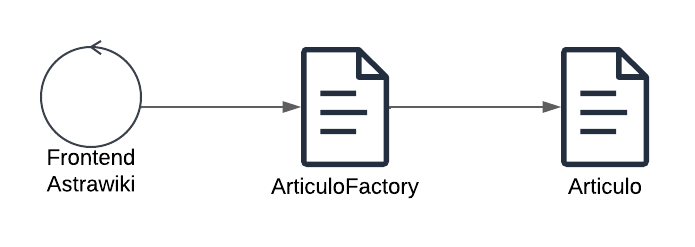
\includegraphics[width=0.5\linewidth]{img/astrawiki-articulo-factory.png}
    \caption{\textit{Smart contracts} que intervienen en el repositorio de conocimiento}
    \label{fig:aw-eth-articulo-factory}
\end{figure}

Ambos casos de uso resultaron muy similares en su resolución. Haciendo uso del patrón de diseño \textit{Factory} existe un smart contract Factory que crea otros smart contracts (Artículo o Chat, según el caso de uso).

\begin{figure}[h]
    \centering
    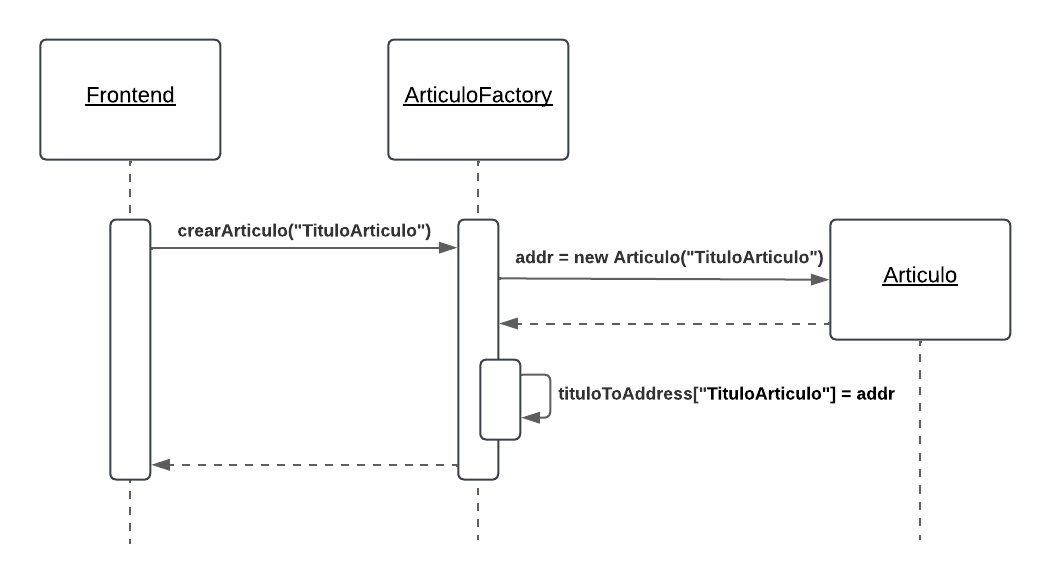
\includegraphics[width=0.75\linewidth]{img/ds-aw-eth-crear-articulo.png}
    \caption{Creación de un artículo}
    \label{fig:ds-aw-eth-crear-articulo}
\end{figure}

De esta manera el \textit{Factory} tiene un \textit{mapping} con todos los articulos creados y las direcciones correspondientes para accederlos. Si se quisiera acceder a un Artículo en particular primero se tiene que consultar al \textit{Factory} para obtener la dirección del mismo y, como cada artículo es un \textit{smart contract} en sí mismo, se puede consultar o modificar su contenido directamente interactuando con el Artículo en particular como se puede ver en la Figura \ref{fig:ds-aw-eth-obtener-contenido-articulo}.

\begin{figure}[h]
    \centering
    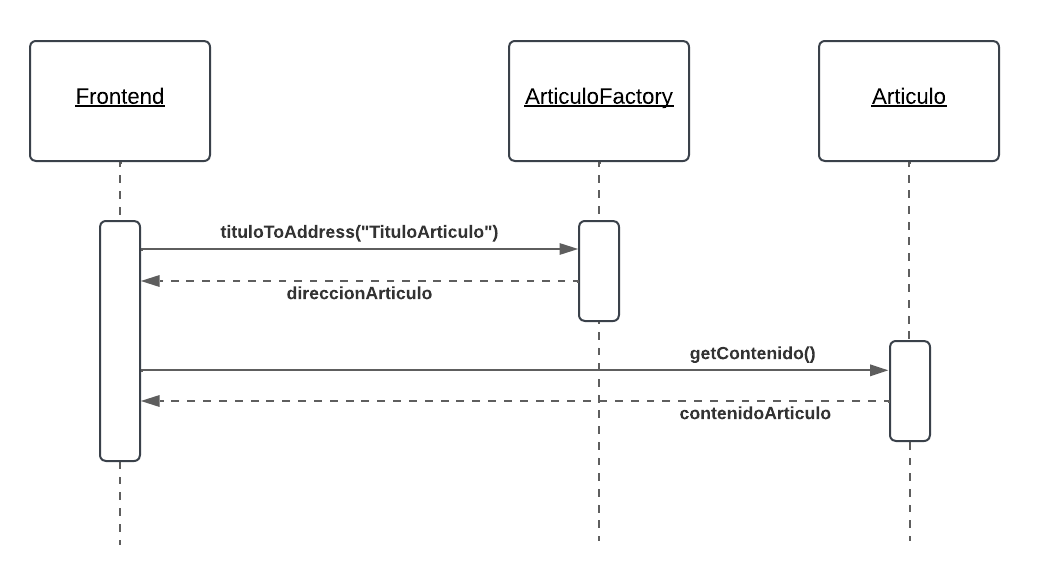
\includegraphics[width=0.75\linewidth]{img/ds-aw-eth-obtener-contenido-articulo.png}
    \caption{Obtención del contenido de un artículo}
    \label{fig:ds-aw-eth-obtener-contenido-articulo}
\end{figure}

La principal diferencia entre el repositorio de conocimiento y el mensajero en tiempo real está en que los mensajes del mensajero tienen que ser vistos por los demás usuarios que participan de la conversación en el momento que se envían. Esto no es estrictamente necesario en el repositorio de conocimiento pero sí lo es en el mensajero.

Para afrontar este requisito se utilizaron los eventos de Solidity (el lenguaje de programación en el que se desarrollan los \textit{smart contract} de Ethereum). Funciona de la siguiente manera, al momento de enviar un mensaje se emite un evento. Este evento se recibe en un listener que fue previamente inicializado al instante previo de haber obtenido el Chat en el frontend. Al recibir este evento el frontend puede actualizar la pantalla mostrando el mensaje nuevo sin necesidad de obtener todos los mensajes.

% TODO: insertar gráfico del flujo de un evento al enviar un mensaje 